%%%%%%%%%%%%%%%%%%%%%%%%%%%%%%%%%%%%%%%%%%%%%%%%%%%%%%%%%%%%%%%%%%%%%%%%%%%%%%%%
%2345678901234567890123456789012345678901234567890123456789012345678901234567890
%        1         2         3         4         5         6         7         8

\documentclass[a4paper, 10pt, conference]{ieeeconf} 
\usepackage{graphicx}
\usepackage{listings}
\usepackage{float}
\title{\LARGE \bf
Visualization module solving logical problems for the FORMULA system
}


\author{Ksenia Panova\\%
 \small Student of Peter the Great\\%
 \small Saint-Petersburg Polytechnic University\\%
 \small Email: k-nazarova@mail.ru}

\begin{document}

\maketitle
\thispagestyle{empty}
\pagestyle{plain}



%%%%%%%%%%%%%%%%%%%%%%%%%%%%%%%%%%%%%%%%%%%%%%%%%%%%%%%%%%%%%%%%%%%%%%%%%%%%%%%%
\begin{abstract}
Visualization programs are used for various purposes (training, debugging and optimization) by programmers. However, such programs are often highly dependent on programming paradigms for which they were created, and not always successfully adapt to the calculations made in other paradigms. This paper describes designed system which intended for data visualization. It focuses on information visualization of solutions of logical problems derived from the FORMULA system.
\end{abstract}

%%%%%%%%%%%%%%%%%%%%%%%%%%%%%%%%%%%%%%%%%%%%%%%%%%%%%%%%%%%%%%%%%%%%%%%%%%%%%%%%
\section{INTRODUCTION}

We have designed the module of visualization of solutions obtained via the smt solver Formula. Solvers for satisfiability modulo theories (SMT) check the satisfiability of first-order formulas containing operations from various theories such as the booleans, bit-vectors, arithmetic. A thorough consideration of various methods of visualization was made. As a result of studies the declarative programming language for solutions of logic problems such as Einstein task or the problem of queens was developed.

\section{PROBLEMS}
The developed system is designed for data visualization. The purpose of the study is to consider an information visualization solutions of logical problems derived from the FORMULA system, which is fundamentally different from existing visualization tools. The most obvious advantage of the new system is that the developed module operates with a much smaller amount of information, which saves time and expense of resources for the visualization process.

The main task of the investigation is to design an integrated module of visualization solutions and the results of logical tasks.

The developed module should maintain the following functions:
\begin{enumerate}
\item Integration module logical solution FORMULA tasks, analysis of the results of using it
\item Display of static solutions with support for the following types of visualization:
\begin{enumerate}
\item Table
\item Counts
\item Vectors
\end{enumerate}
\item Display of the process of solving problems by means of a dynamic visualization:
\begin{enumerate}
\item Moving objects
\item Time Management
\end{enumerate}
\end{enumerate}

\section{ARCHITECTURE DESIGN}

The project structure is shown in Fig.~\ref{fig:structure}
The system is a program running in Windows. It analyzes configured via FORMULA file, and loads the content to the respective variable depending on the type of task and the format:
\begin{itemize}
\item For a static display in a table - table
\item For dynamic display - sequence
\end{itemize}
\begin{figure}[h]
    \centering
    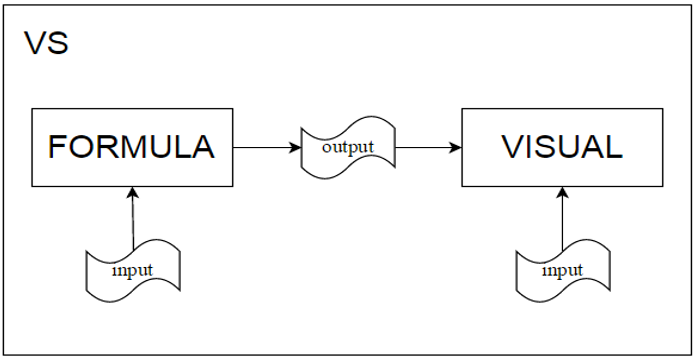
\includegraphics[width=0.4\textwidth]{structure.png}
    \caption{Project structure}
    \label{fig:structure}
\end{figure}

The first component of this structure - FORMULA system, in which the task of first-order logic is implemented and executed. This step tests satisfiability of task, and if it is, the result is written to the output file. Visualization system uses this file to obtain the solution of the proposed problem and its graphical display.\\


\section{LANGUAGE MODULE}
Starting the system designed by the programming language is accompanied by its conversion into a form that is meaningful to the computer. Therefore, we need a program that reads the text written in one language (the source) and translates it into an equivalent text in another language.
\begin{itemize}
\item For a static display in a table - table
\item For dynamic display - sequence
\end{itemize}
\begin{figure}[h]
    \centering
    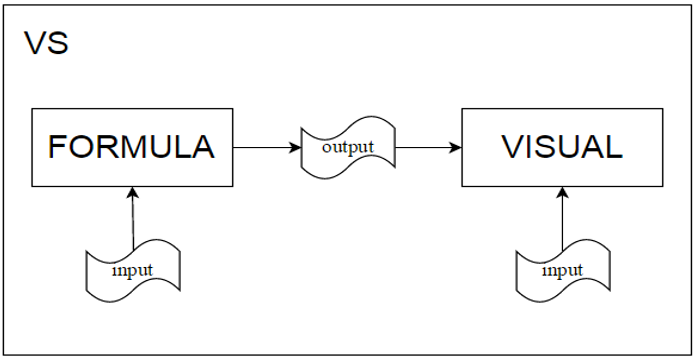
\includegraphics[width=0.4\textwidth]{structure.png}
    \caption{Project structure}
    \label{fig:structure}
\end{figure}

In order to provide this, compiler that converts a program written in the language of visualization, in a program written in C ++ was developed.

For that, lexer performs lexical analysis which is the process of converting a sequence of characters  into a sequence of tokens (strings with an identified "meaning"). Lexical analysis was performed using parser generator "Lex".

After lexical analysis is the syntactic analysis. Parsing or syntactic analysis is the process of analysing a string of symbols, either in natural language or in computer languages, conforming to the rules of a formal grammar. The purpose of syntactic analysis is to determine the structure of the input text. This structure consists of a hierarchy of phrases, the smallest of which are the basic symbols and the largest of which is the sentence\cite{c1}. The structure can be described by a tree with one node for each phrase. Basic symbols are represented by values stored at the nodes. The root of the tree represents the sentence. an example is shown in Fig.~\ref{fig:parsetree}. Syntactic analysis was performed using generator "Yacc", which provides automatic construction of grammatical analysis procedures.

As a result of the joint compilation of the generated lexer and parser , executable file visual.exe is created for handling of code with new syntax.

\begin{figure}[h]
    \centering
    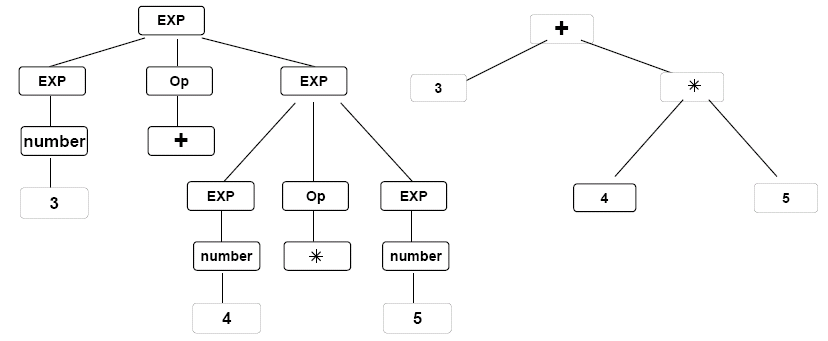
\includegraphics[width=0.5\textwidth]{parsetree.png}
    \caption{Example of syntactic analysis}
    \label{fig:parsetree}
\end{figure}

The code generator solves the basic problem of the translator: in the process of traversal of the syntax tree it takes tokens in the machine instruction sequence. Tokens are extracted from the tree nodes in a certain order . When the amount of tokens is enough to determine the desired operation, code generator generates corresponding machine instructions and tree traversal resumes.

Connectivity between Lex and Yacc is shown in Fig.~\ref{fig:generation}.

\begin{figure}[h]
    \centering
    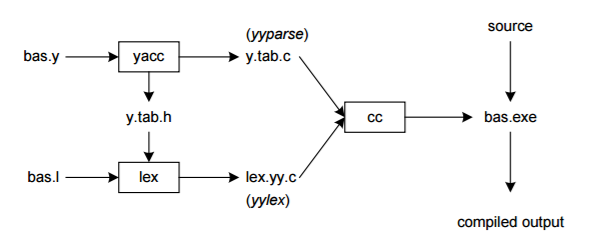
\includegraphics[width=0.5\textwidth]{generation.png}
    \caption{Building a Compiler with Lex/Yacc}
    \label{fig:generation}
\end{figure}

Yacc reads the grammar descriptions in bas.y and generates a syntax analyzer (parser), that includes function yyparse, in file y.tab.c. Included in file bas.y are token declarations. Also yacc generates definitions for tokens and places them in file y.tab.h. Lex reads the pattern descriptions in bas.l, includes file y.tab.h, and generates a lexical analyzer, that includes function yylex, in file lex.yy.c.

Finally, the lexer and parser are compiled and linked together to create executable bas.exe. Then we call yyparse to run the compiler. Function yyparse automatically calls yylex to obtain each token\cite{c2}.

\section{SYNTAX}
Alphabet of the visualization language consists of latin alphabet letters (uppercase and lowercase), underscores, arabic numerals, and special characters (- + =, {} () []!). This syntax is case sensitive.
\begin{lstlisting}
<name> = (<letter>|_)
	 {<letter>|<letter>|_}
<letter> = A|B|...|Y|Z|a|b|...|y|z
<digit> = 0|1|...|9
\end{lstlisting}
As identity is unacceptable to use the reserved keywords that have an impact on the translator and are used to form a variety of language structures, or which are the names of standard functions:
\textit{print, show, move, backgnd, slab, table, listing, if, foreach, in}.\\

In the statement, all the tokens can be separated by any number of whitespace characters, which includes spaces, tabs, and newline, carriage return, and newline.

Conditions:
\begin{lstlisting}
if  (<condition>)
	<statement>
\end{lstlisting} or
\begin{lstlisting}
if  (<condition>)
	<statement>
else
	<statement>
\end{lstlisting}
Enumeration is used to declare all imaging facilities:
\begin{lstlisting}
enum <enum_name>{<item>, <item>, ...};
\end{lstlisting}

The syntax allows one-dimensional and two-dimensional arrays consisting of sets of integers or strings. Moreover, one-dimensional arrays can be of different types.

\begin{enumerate}
\item Standard one-dimensional array
\begin{lstlisting}
<array_name>[<size>] = 
	{<statement>, ...};
\end{lstlisting}
\item A one-dimensional array associated with a list of visualization objects, which consist of a set of strings, namely paths to images of the respective objects
\begin{lstlisting}
<array_name>[<enum_name>] = 
	{<path>, ...};
\end{lstlisting}
\item A one-dimensional array consisting of a set of pairs of values of the object and its initial state, required to initiate dynamic visualization
\begin{lstlisting}
<pair> = (<object_name>,<init_state>)
<array_name>[<size>] = 
	{<pair>, ...};
\end{lstlisting}
\item Two-dimensional array
\begin{lstlisting}
<array_name>[<size>][<size>] = {
	<statement>,...;
	<statement>,...;
	...
};
\end{lstlisting}
\end{enumerate}

Also, the syntax requires a foreach statement, which defines a cyclic structure, repeating groups of operators in relation to each element of the array.
\begin{lstlisting}
foreach (<item> in <array_name>)
	<statement>
\end{lstlisting}

One of the standard functions is print, which prints the value received on its input variable to standard output:
\begin{lstlisting}
print <name>;
\end{lstlisting}

To determine the format of the visualization, dynamic or static (table), keywords \textit{table} and \textit{sequence} are used. \textit{table} is the ID of a two-dimensional array, which is loaded from the result of the FORMULA, \textit{sequence} - a standard function that initializes the dynamic visualization.

The function \textit{sequence} takes two arguments:
\textbf{operator} is the number of states between which the transitions, and \textbf{array\_name} is identifier of the array that contains the objects for display and their initial states.
\begin{lstlisting}
sequence (<statement>, <array_name>);
\end{lstlisting}

Standard function \textit{move} is used to switch between the states. \textit{move} obtains object name, which should change its current state. The direction of movement of the object is based on the previous states.
\begin{lstlisting}
move(<object_name>);
\end{lstlisting}

The primary function of language is function for downloading of the format and objects into visualizer and graphical representation of these objects. This role performs the function \textit{show}:
\begin{lstlisting}
<show_statement> = table |
	sequence (<statement>,
		<array_name>) |
	move(<object_name>);
show <show_statement>;
\end{lstlisting}

\section{VISUALIZATION MODULE}
A key part of the system architecture is graphical module. As a GUI library use Qt 5.4.1 - cross-platform toolkit software development with C ++ programming.\\
The following classes are the basis of the implementation of the visualization module:
\begin{enumerate}
\item Class \textit{Visual} - a class that is responsible for the display of objects in the dialog box.
\item Class \textit{NewItem} - a class that is responsible for a separate display object, describes its size, location, and its direction of movement in the case of dynamic visualization.
\item Class \textit{NewState} - a class inherited from QGraphicsItem  which describes a separate state, its size and location in the dialog box. It is used in dynamic imaging.
\item Class \textit{MakeMove} - a class that initiates the download of status objects and their movement when dynamic visualization.
\item Class \textit{NewTable} - a class inherited from QGraphicsItem. It describes and visualizes the table.

UML diagram of this module in Fig.~\ref{fig:uml}.\\
\begin{figure}[h]
    \centering
    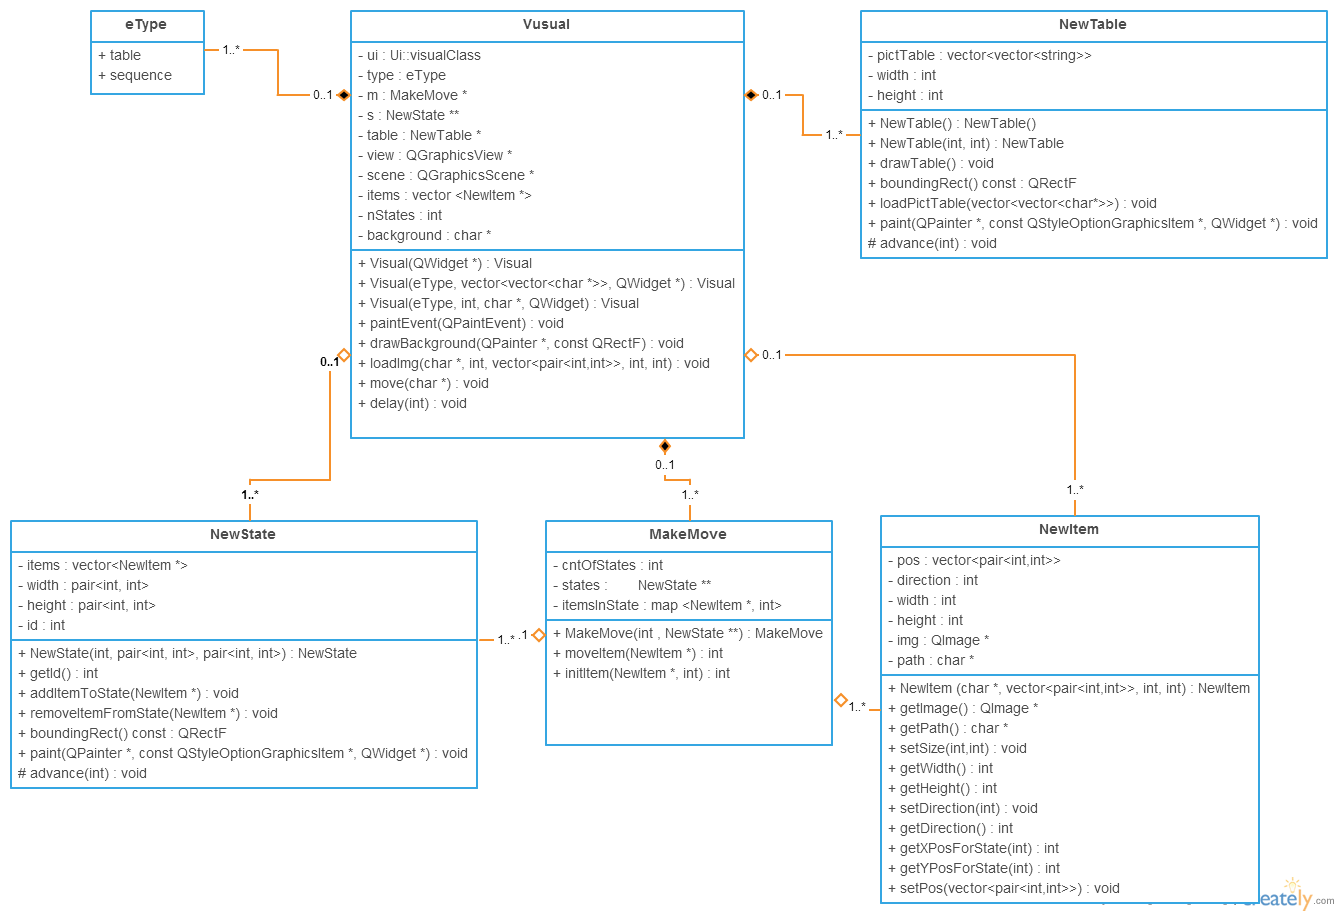
\includegraphics[width=0.5\textwidth]{uml.png}
    \caption{UML diagram of visualization module}
    \label{fig:uml}
\end{figure}
%\begin{itemize}
%\item Default constructor
%\begin{lstlisting}
%Visual(QWidget *parent = 0);
%\end{lstlisting}	
%\item Constructor that initializes and starts rendering the table
%\begin{lstlisting}
%Visual(eType type,
%	vector<vector<char *>>&v,
%	QWidget *parent = 0);
%\end{lstlisting}	
%\item Constructor that initializes the process of dynamic visualization: specifies the number of initial states
%\begin{lstlisting}
%Visual(eType type,
%	int nStates,
%	char *bg = NULL,
%	QWidget *parent = 0);
%\end{lstlisting}	
%\item Destructor
%\begin{lstlisting}
%~Visual();
%\end{lstlisting}	
%\item Drawing the background
%\begin{lstlisting}
%void drawBackground(QPainter *painter,
%	const QRectF &rect);
%\end{lstlisting} 	
%\item Loading of mappings, their sizes, coordinates and initial states
%\begin{lstlisting}
%void loadImg(char *path,
%	int initState,
%	vector<pair<int,int>>&v,
%	int w=100, int h=100);
%\end{lstlisting}	
%\item Moving an object to another state
%\begin{lstlisting}
%void move(char *img);
%\end{lstlisting}	
%\item Delaying
%\begin{lstlisting}
%void delay(int sec);
%\end{lstlisting}
%\end{itemize}

\end{enumerate}

\section{TESTING}
Consider the example of visualization of Einstein problem.

\textbf{Task:}
5 different people live in 5 houses of different colors, smoke 5 different brands of cigarettes, look after 5 different animals, drink 5 different beverages.
At the same time, there are 15 conditions:
\begin{enumerate}
\item The Norwegian lives in the first house.
\item The Englishman lives in the red house.
\item The green house is immediately to the left of the white.
\item The Dane drinks tea.
\item The one who smokes Rothmans, lives next to the one who has cat.
\item Anyone who lives in the yellow house smokes Dunhill.
\item The German smokes Marlboro.
\item He who lives in the center drinks milk.
\item A neighbor of the one who smokes Rothmans, drinks water.
\item The man who smokes Pall Mall, has bird.
\item The Swede has dog.
\item The Norwegian lives next to the blue house.
\item Whoever has horse lives in the blue house.
\item The man who smokes Philip Morris, drinking beer.
\item In the green house drinks coffee.
\end{enumerate}

\textbf{Question:} Who has fish?

\textbf{Result} of visualization is static  table with the solution of the problem. Here see that the owner of fish is the German (Fig.~\ref{fig:test}):

\begin{figure}[H]
    \centering
    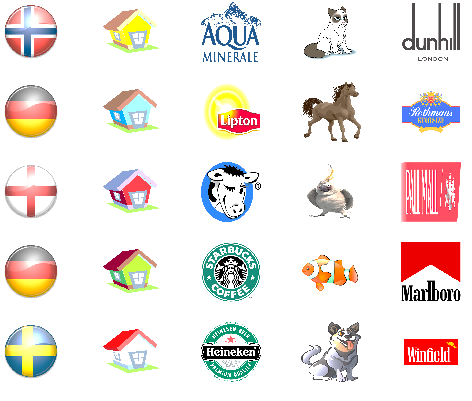
\includegraphics[width=0.5\textwidth]{test.png}
    \caption{Result visualization solutions of Einstein's problem}
    \label{fig:test}
\end{figure}

\section{CONCLUSIONS}

As a result of studies the integrated module of visualization solutions and the results of logical tasks was designed. Also visualization language was developed. For that rules and  a new programming language syntax  have been formulated, on the basis of which carried out the lexical, syntactic and semantic analysis. Graphical system module is also designed to visualize input data in a predetermined format, namely in the form of static and dynamic table moving objects.   

\addtolength{\textheight}{-12cm}

\begin{thebibliography}{99}

\bibitem{c1} A. Aho, M. Lam, R. Sethi, Compilers: Principles, Techniques, and Tools, 2008.
\bibitem{c2} T. Niemann, Lex \& Yacc tutorial.

\end{thebibliography}

\end{document}
